\section{Introduction to Work}

\begin{definition}{def4.1:label}
    \textbf{WORK: How much energy it takes to do a certain physical action.}

    $$
    W = \Delta E = \vec F \cdot \vec {\Delta x}
    $$

    $W$ = Work done (SI Units: $\J = \N\m$)\\
    $\Delta E$ = Change in energy\\
    $\vec F$ = the force applied\\
    $\Delta x$ = the displacement over which the object was applied the given force $\vec F$
\end{definition}


\begin{problem}
    A couch is pushed with a force 25 $\N$ over a distance of 5 $\m$. Calculate the work that is applied to the couch. 

    $$
    \begin{aligned}
        W &= F_A \cdot \Delta x\\
        W &= (25 \N)(5 \m)\\
        W &= 100 \J
    \end{aligned}
    $$
\end{problem}


\begin{problem}
    \textbf{SEE ATTACHED FIGURE}

    a) How much energy is expended by the applied force to move the couch 5 $\m$?
    b) How much energy does the frictional force expend to move the couch 5 $\m$?

    To solve part a):
    $$
    \begin{aligned}
        W_A &= F_{Ax} \cdot \Delta x\\
        W_A &= F\cos\theta \cdot \Delta x\\
        W_A &= (50 \N)\cos(25^\circ)(5 \m)\\
        W_A &= 227 \J
    \end{aligned}
    $$

    To solve part b):
    $$
    \begin{aligned}
        W_f &= -F_f \cdot \Delta x\\
        W_f &= -\mu_kF_N \cdot \Delta x\\
        W_f &= -\mu_k(mg + F_A\sin\theta) \cdot \Delta x\\
        W_f &= -(0.15)((20\kg)(9.81\frac{\m}{\s^2}) + (50\N)\sin(25^\circ))
        W_f &= VALUE
    \end{aligned}
    $$
\end{problem}


\section{Energy}

Energy comes in many different forms. The main forms of energy (as well as the proofs to get their respective equations) are listed below:


\begin{definition}[Kinetic Energy]{def4.2:label}
    If an object is moving, the energy that the object expends is equal to the \textbf{kinetic energy}. 

    $$
    KE = \frac{1}{2}mv^2
    $$

    $KE$ = the kinetic energy expended\\
    $m$ = mass of the object\\
    $v$ = velocity of the object at the given moment where you wish to find the energy
\end{definition}

\begin{proof}
    PROOF OF KINETIC ENERGY HERE
\end{proof}


\begin{definition}[Potential Energy]{def4.3:label}
    $$
    PE = mgh
    $$
\end{definition}

\begin{proof}
    PROOF OF POTENTIAL ENERGY HERE
\end{proof}

\begin{definition}[Spring Energy]{def4.4:label}
    $$
    SE = \frac{1}{2}kx^2
    $$
\end{definition}

\begin{proof}
    PROOF OF SPRING ENERGY HERE
\end{proof}

\textbf{NOTE:} Energy is \textit{positive} if energy is being stored and \textit{negative} if energy is being released.

\subsection{The Usefulness of Energy and Work}

While we have an equation for the work if we know the applied forces, if we know other elements about the system (how fast ) [FINISH THIS LATER]


\begin{problem}
    ADD PROBLEM TEXT LATER

    \begin{center}
        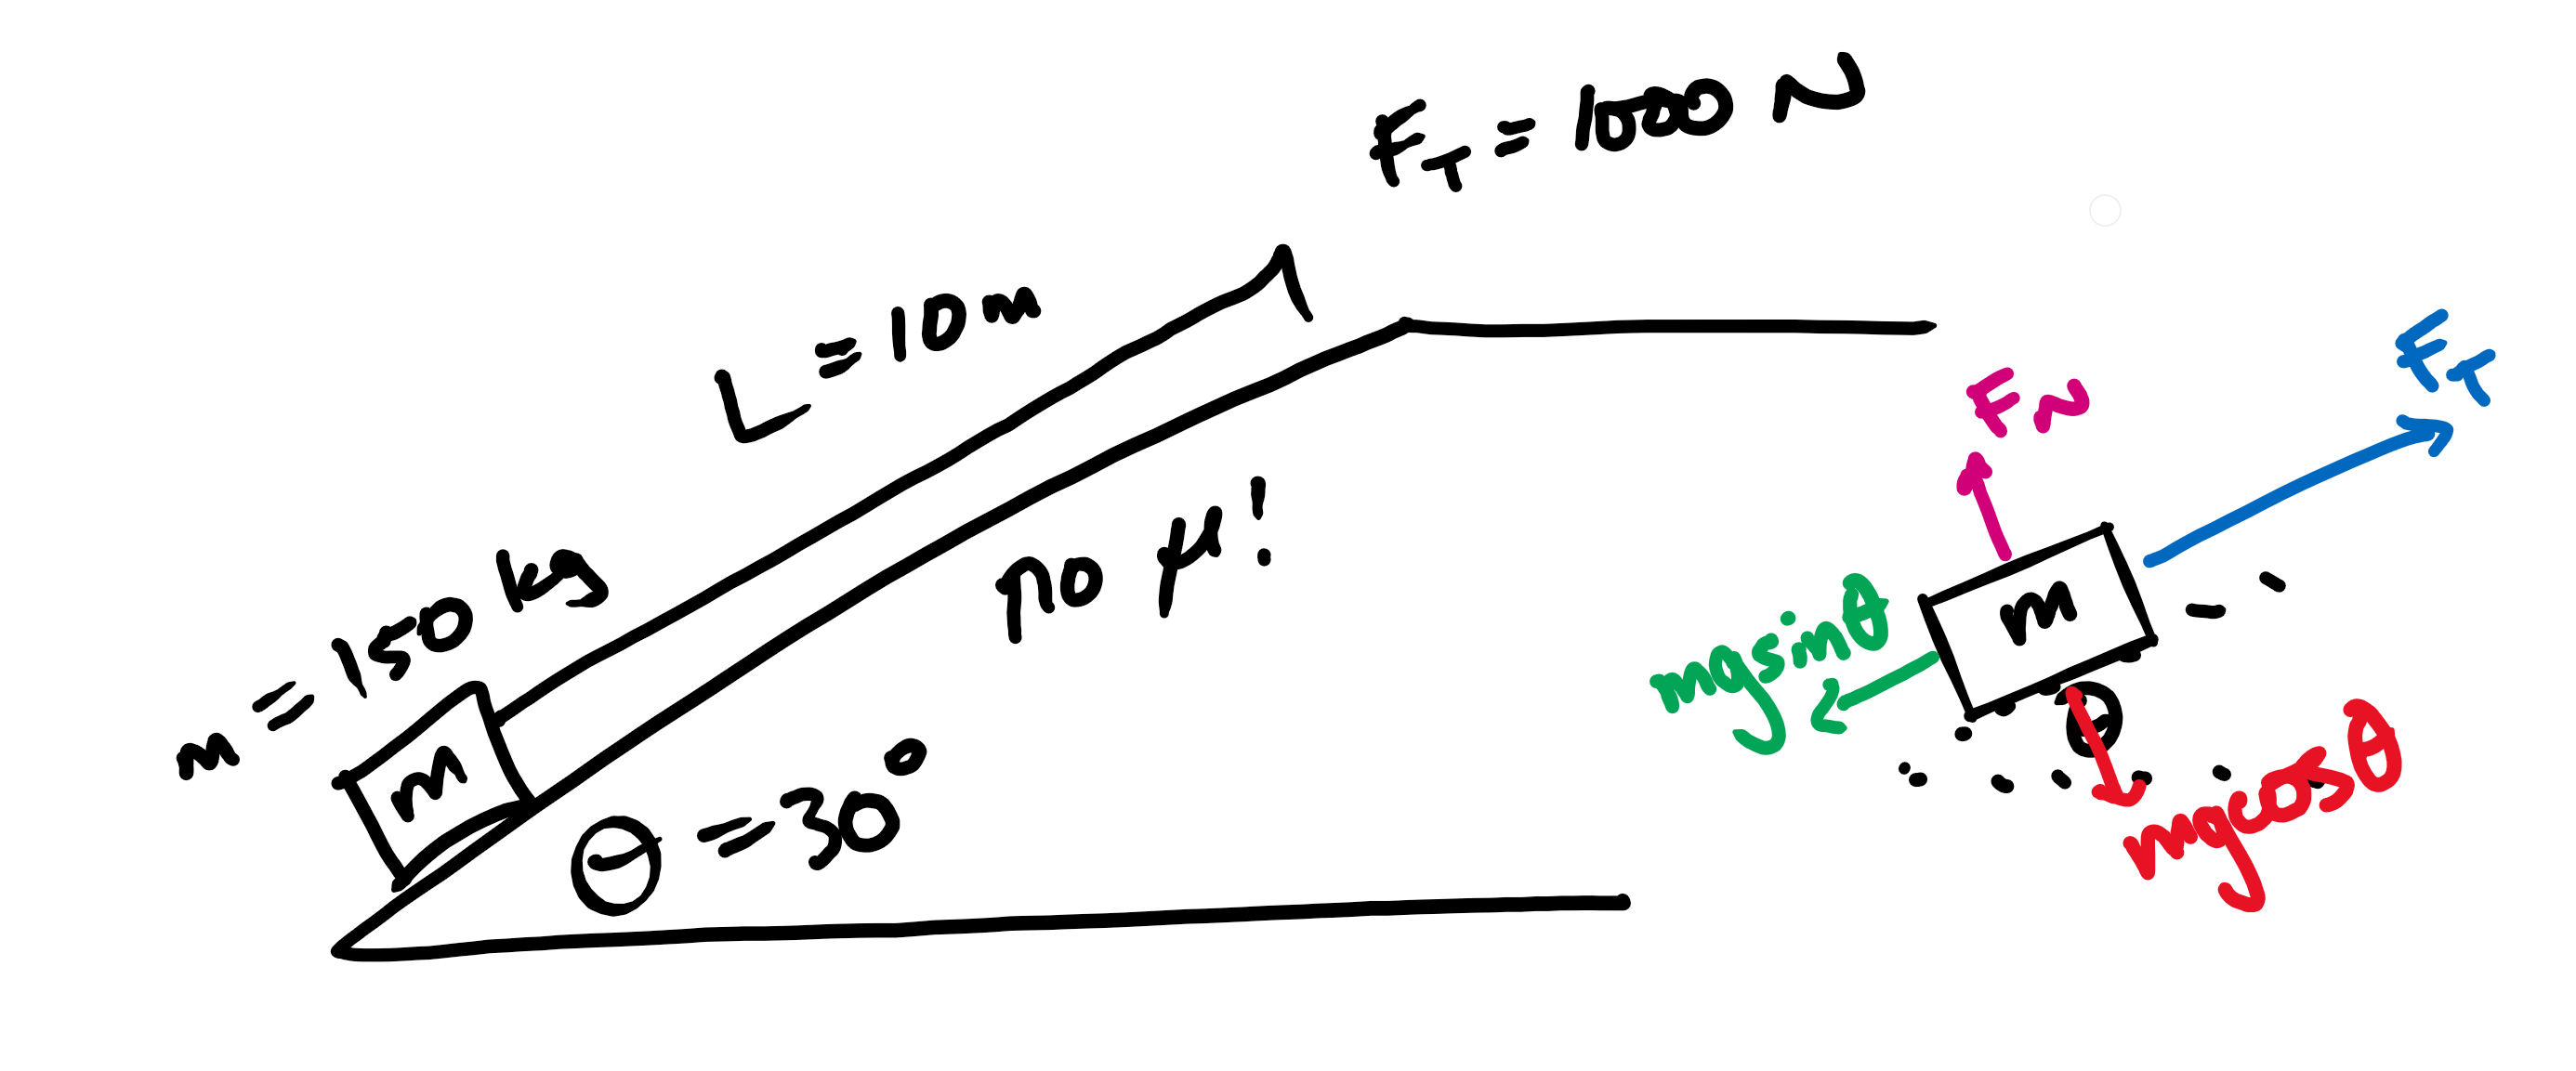
\includegraphics[width=0.5\textwidth]{chapters/ch4/images/fig4_5.PNG}
    \end{center}

    While this problem could be solved using kinematics and Newton's second law, we can also use the Work-Energy theorem. 

    $$
    \begin{aligned}
        W_{in} &= \Delta KE + \Delta PE\\
        F_T \cdot L &= \frac{1}{2}m(v_f - v_i)^2 + mg(h_f - h_i)\\
        F_T \cdot L &= \frac{1}{2}mv_f^2 + mgh_f\\
        v_f &= \sqrt{\frac{2(F_TL - mgh_f)}{m}}\\
        v_f &= \sqrt{\frac{2(F_TL - mg(L\sin\theta))}{m}}
    \end{aligned}
    $$
\end{problem}

\begin{problem}
    A skiier starts at the top of a mountain and is attached a spring at the bottom of the cliff. The skiier will also experience friction for 15m at the bottom of the slope right before the spring. How far was the spring compressed when the skiier reaches the bottom of the slope?

    \begin{center}
        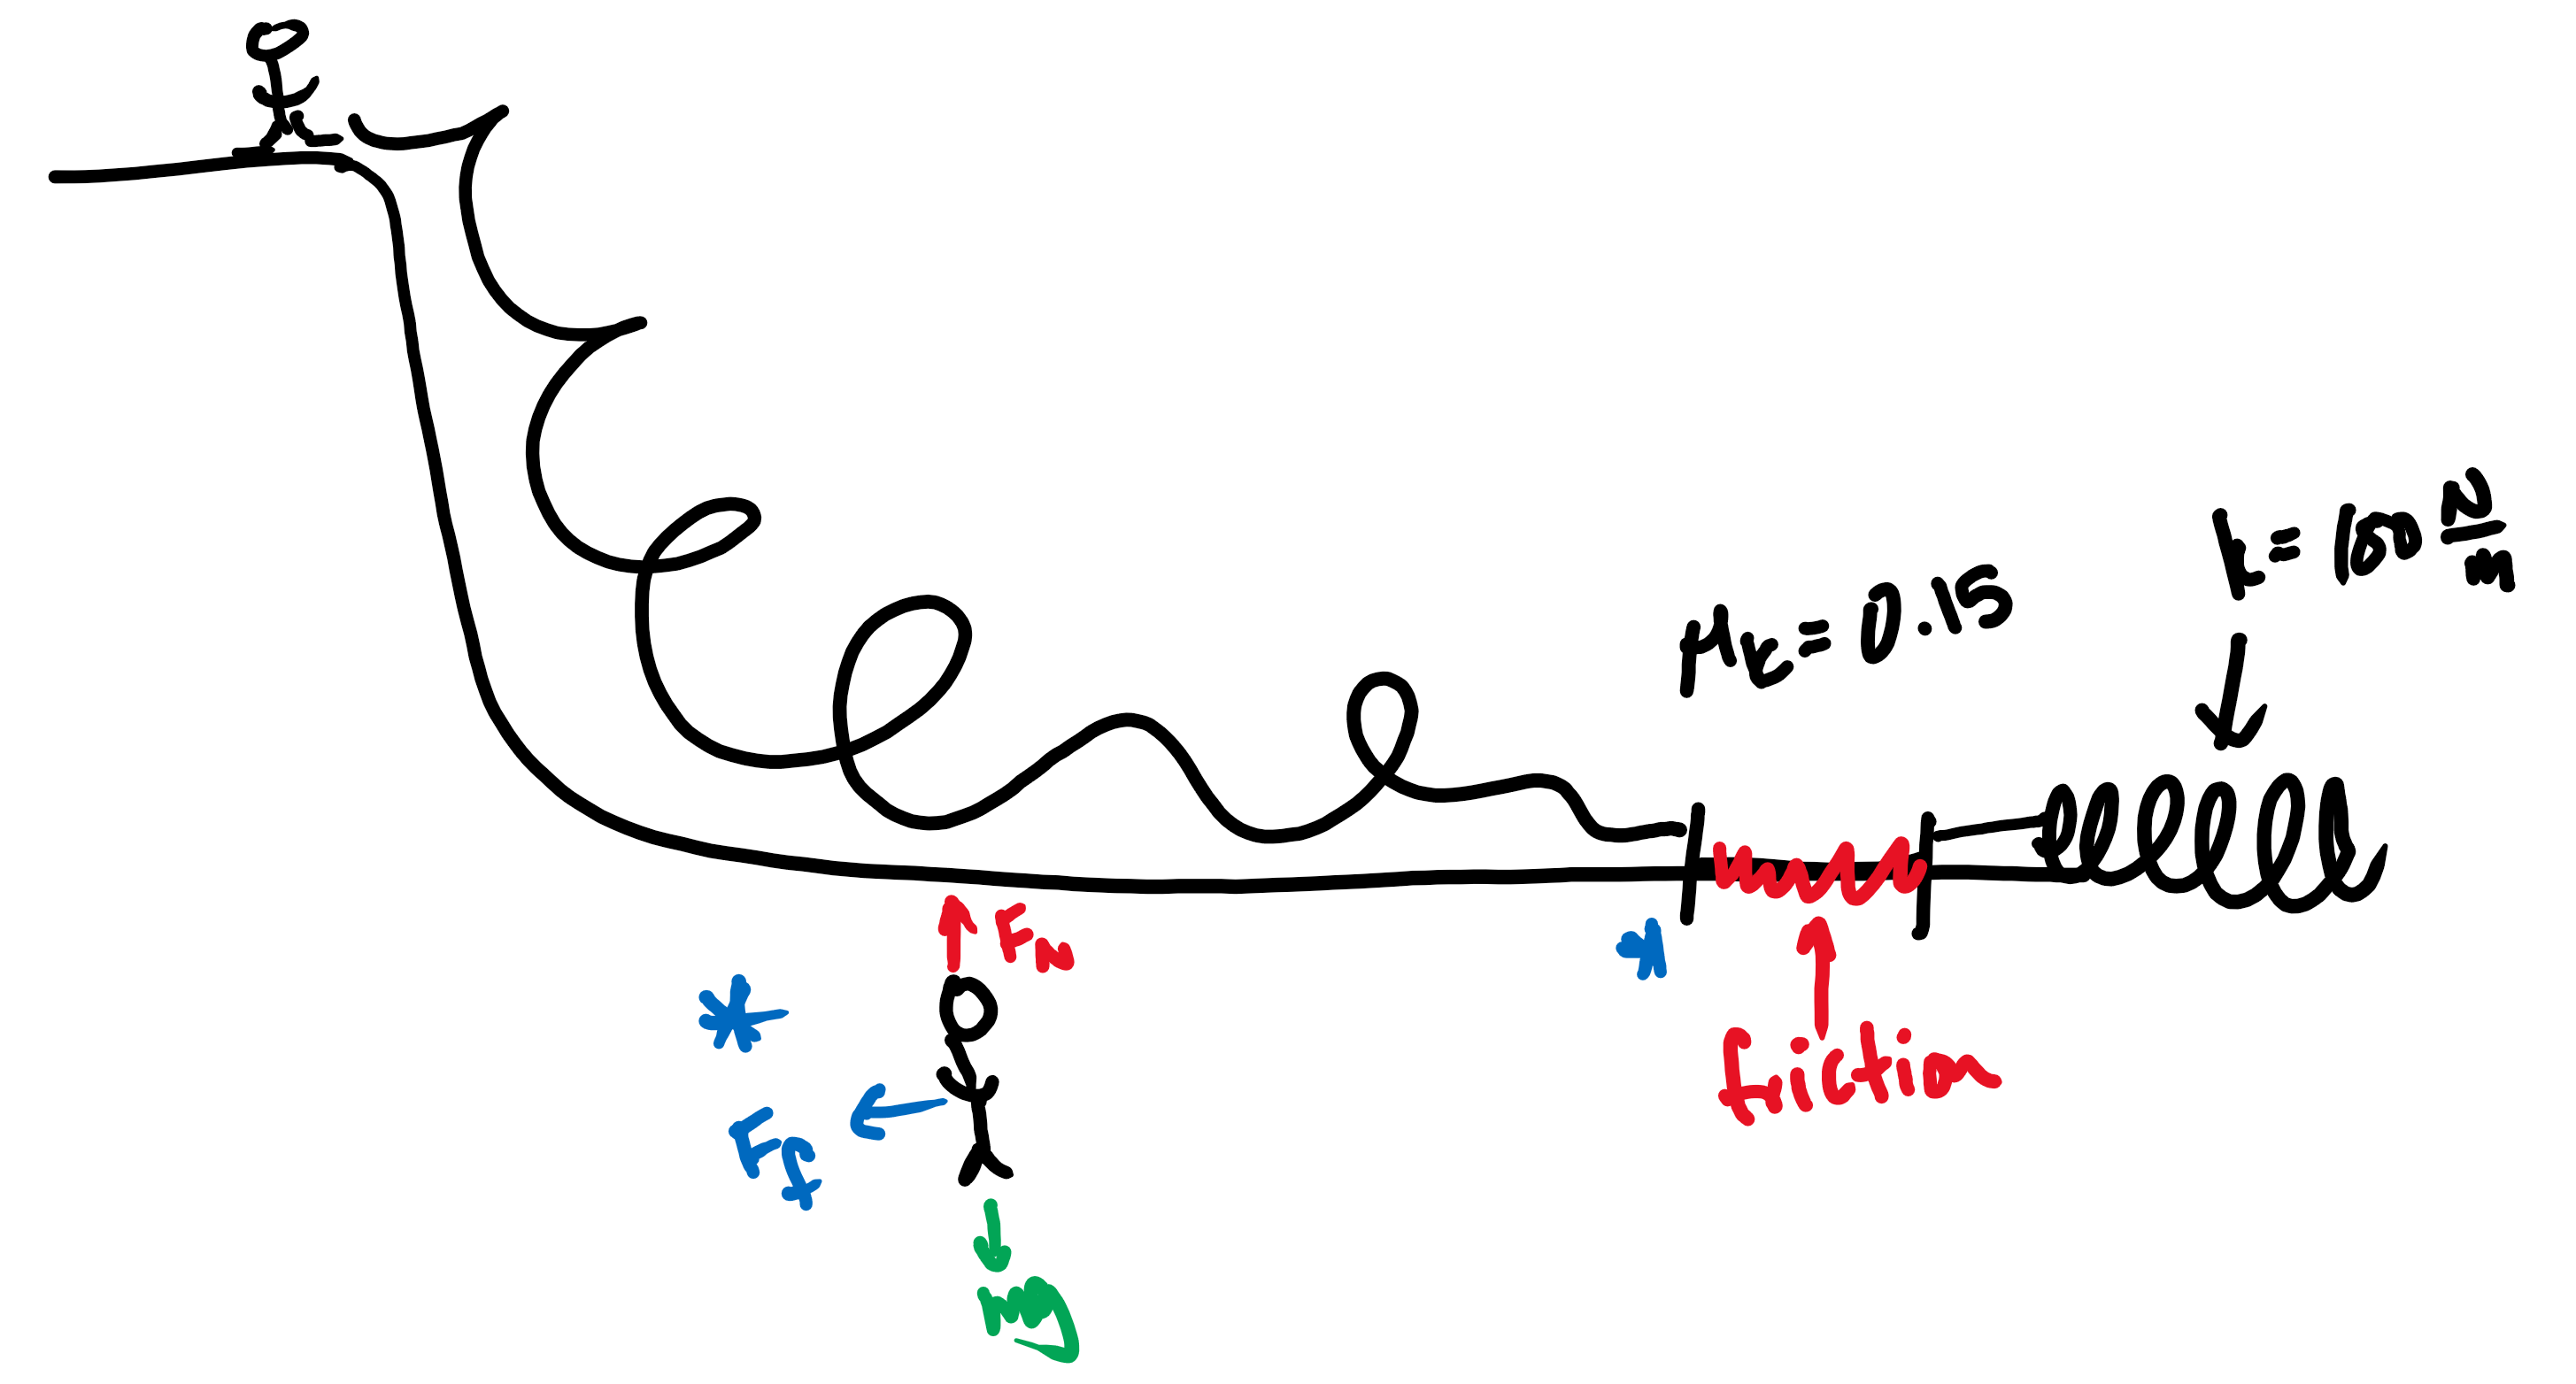
\includegraphics[width=0.5\textwidth]{chapters/ch4/images/fig4_6.PNG}
    \end{center}

    $$
    \begin{aligned}
        W_{in} = 0 &= \Delta PE + \Delta E_s + \Delta E_{T}\\
        0 &= mg(h_f-h_i) + \frac{1}{2}k(x_f-x_i)^2 + \mu_kmgD\\
        0 &= -mgh_i + \frac{1}{2}kx_f^2 + \mu_kmgD\\
        x_f &= \sqrt{\frac{(mgh_i-\mu_kmgD)^2}{k}}\\
        x_f &= \sqrt{\frac{((70\kg)(9.81\frac{\m}{\s^2})(50\m)-(0.15)(70\kg)(9.81\frac{\m}{\s^2})(15\m))^2}{150 \frac{\N}{\m}}}\\
    \end{aligned}
    $$
\end{problem}


\begin{problem}
    A stunt artist was launched out of a cannon on a 20m pedestal. He will land in a bucket attached to a pulley. The pulley also has a 50kg mass attached to it, and the bucket is 10m above the ground. Assume the bucket has no mass and the pulley exerts no friction on the string wrapped around the pulley. What is the speed of the stunt artist right when he lands in the bucket? 
    
    \begin{center}
        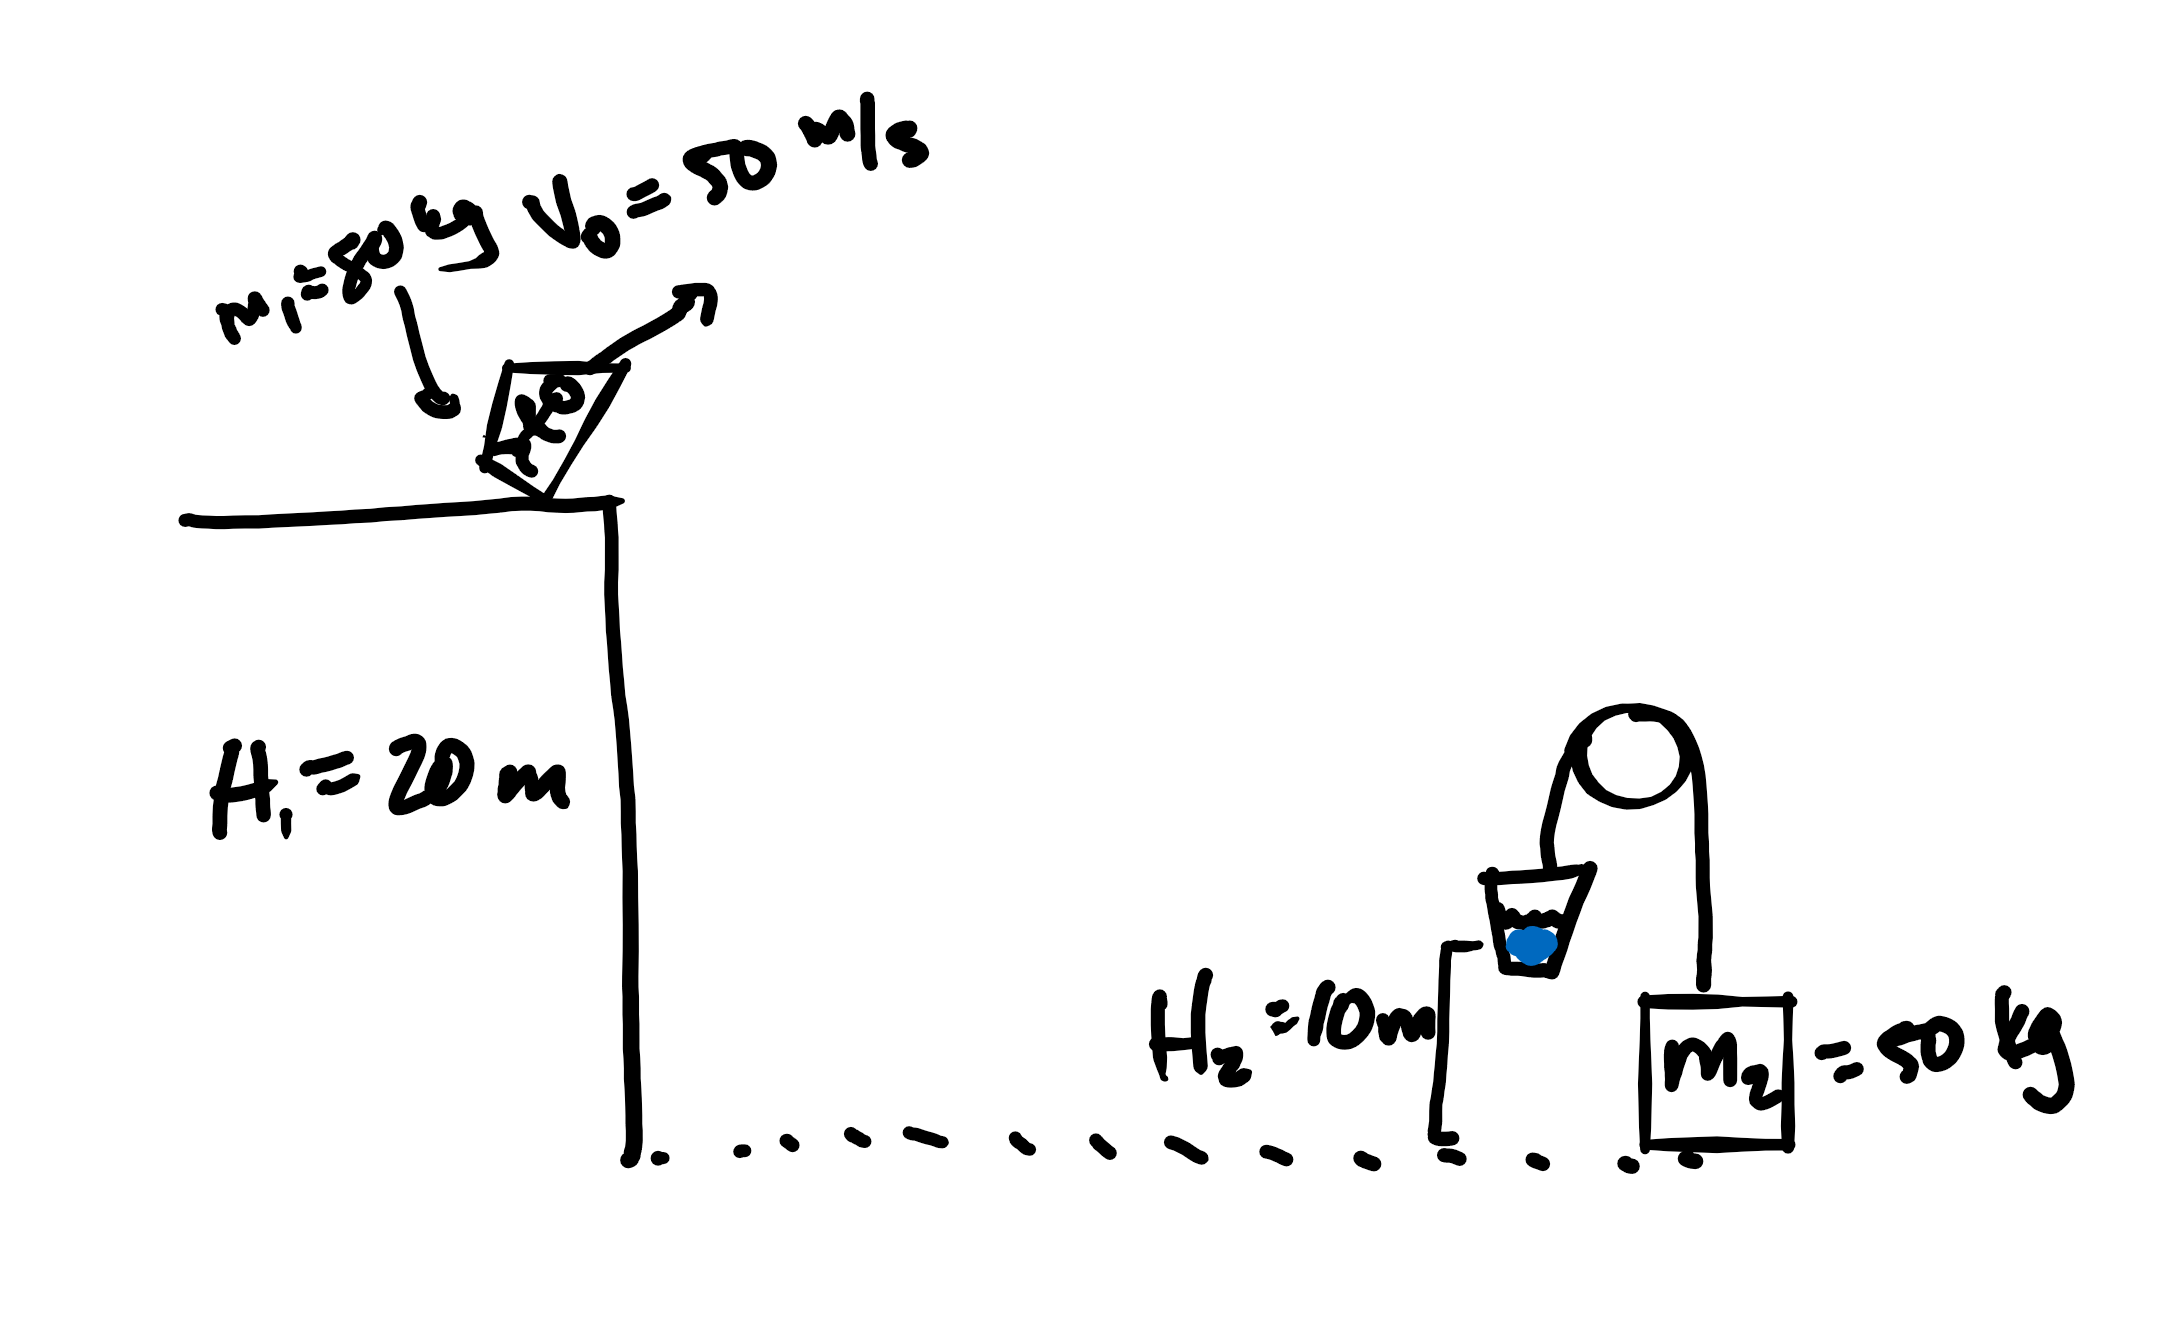
\includegraphics[width=0.5\textwidth]{chapters/ch4/images/fig4_7.PNG}
    \end{center}

    $$
    \begin{aligned}
        W = 0 &= \Delta KE_1 + \Delta PE_1 + \Delta KE_2 + \Delta PE_2\\
        0 &= \frac{1}{2}m(v_{f1}-v_{i1})^2 + \frac{1}{2}m_2(v_{f2}-v_{i2})^2 + m_1g(H_{f1} - H_{i1}) + m_2g(H_{f2} - H_{i2})\\
    \end{aligned}
    $$

    ANSWER: $41.3 \frac{\m}{\s}$
\end{problem}


\section{Work and Calculus}

\begin{itemize}
    \item Sometimes, the force being applied to an object over a given distance is variable
    \item If you are given an equation for what the force is (dependent on distance), then $W = \int_{x_i}^{x_f} F(x) dx$
\end{itemize}


\begin{problem}
    If the force applied to an object (as a function of distance) is $F(x) = 5 - 2x$, what is the work done on the object if the object moves 3 \m?

    $$
    \begin{aligned}
        W &= \int_{x_i}^{x_f} F(x) \: dx\\
        W &= \int_{0}^{3} 5-2x \: dx\\
        W &= (5-2(3))-(5-2(0)) = -1-5
        W &= -6 \J
    \end{aligned}
    $$
\end{problem}


\section{Power}

\begin{definition}[Power]{def4.5:label}
    \textbf{Power:} How much energy is expended over a given time interval.

    $$
    P = \frac{\Delta E}{\Delta t} = \frac{W}{t}
    $$

    \textbf{SI Units:} Watts (W)
\end{definition}


\begin{definition}[Instantaneous Power]{def4.6:label}
    If power is rewritten as a function of time $P(t)$, then:

    $$
    E = \int_{t_1}^{t_2} P(t)dt 
    $$

    Likewise, if you want to find the instantaneous power, then:

    $$
    P(t) = \frac{dE}{dt}
    $$
\end{definition}


\begin{problem}
    A block of mass 1000 kg is attached to a pulley at the top of a building. The pulley is attached to a motor that uses 200 kW. What is the final velocity of the block the moment it reaches the top of the building?

    \begin{center}
        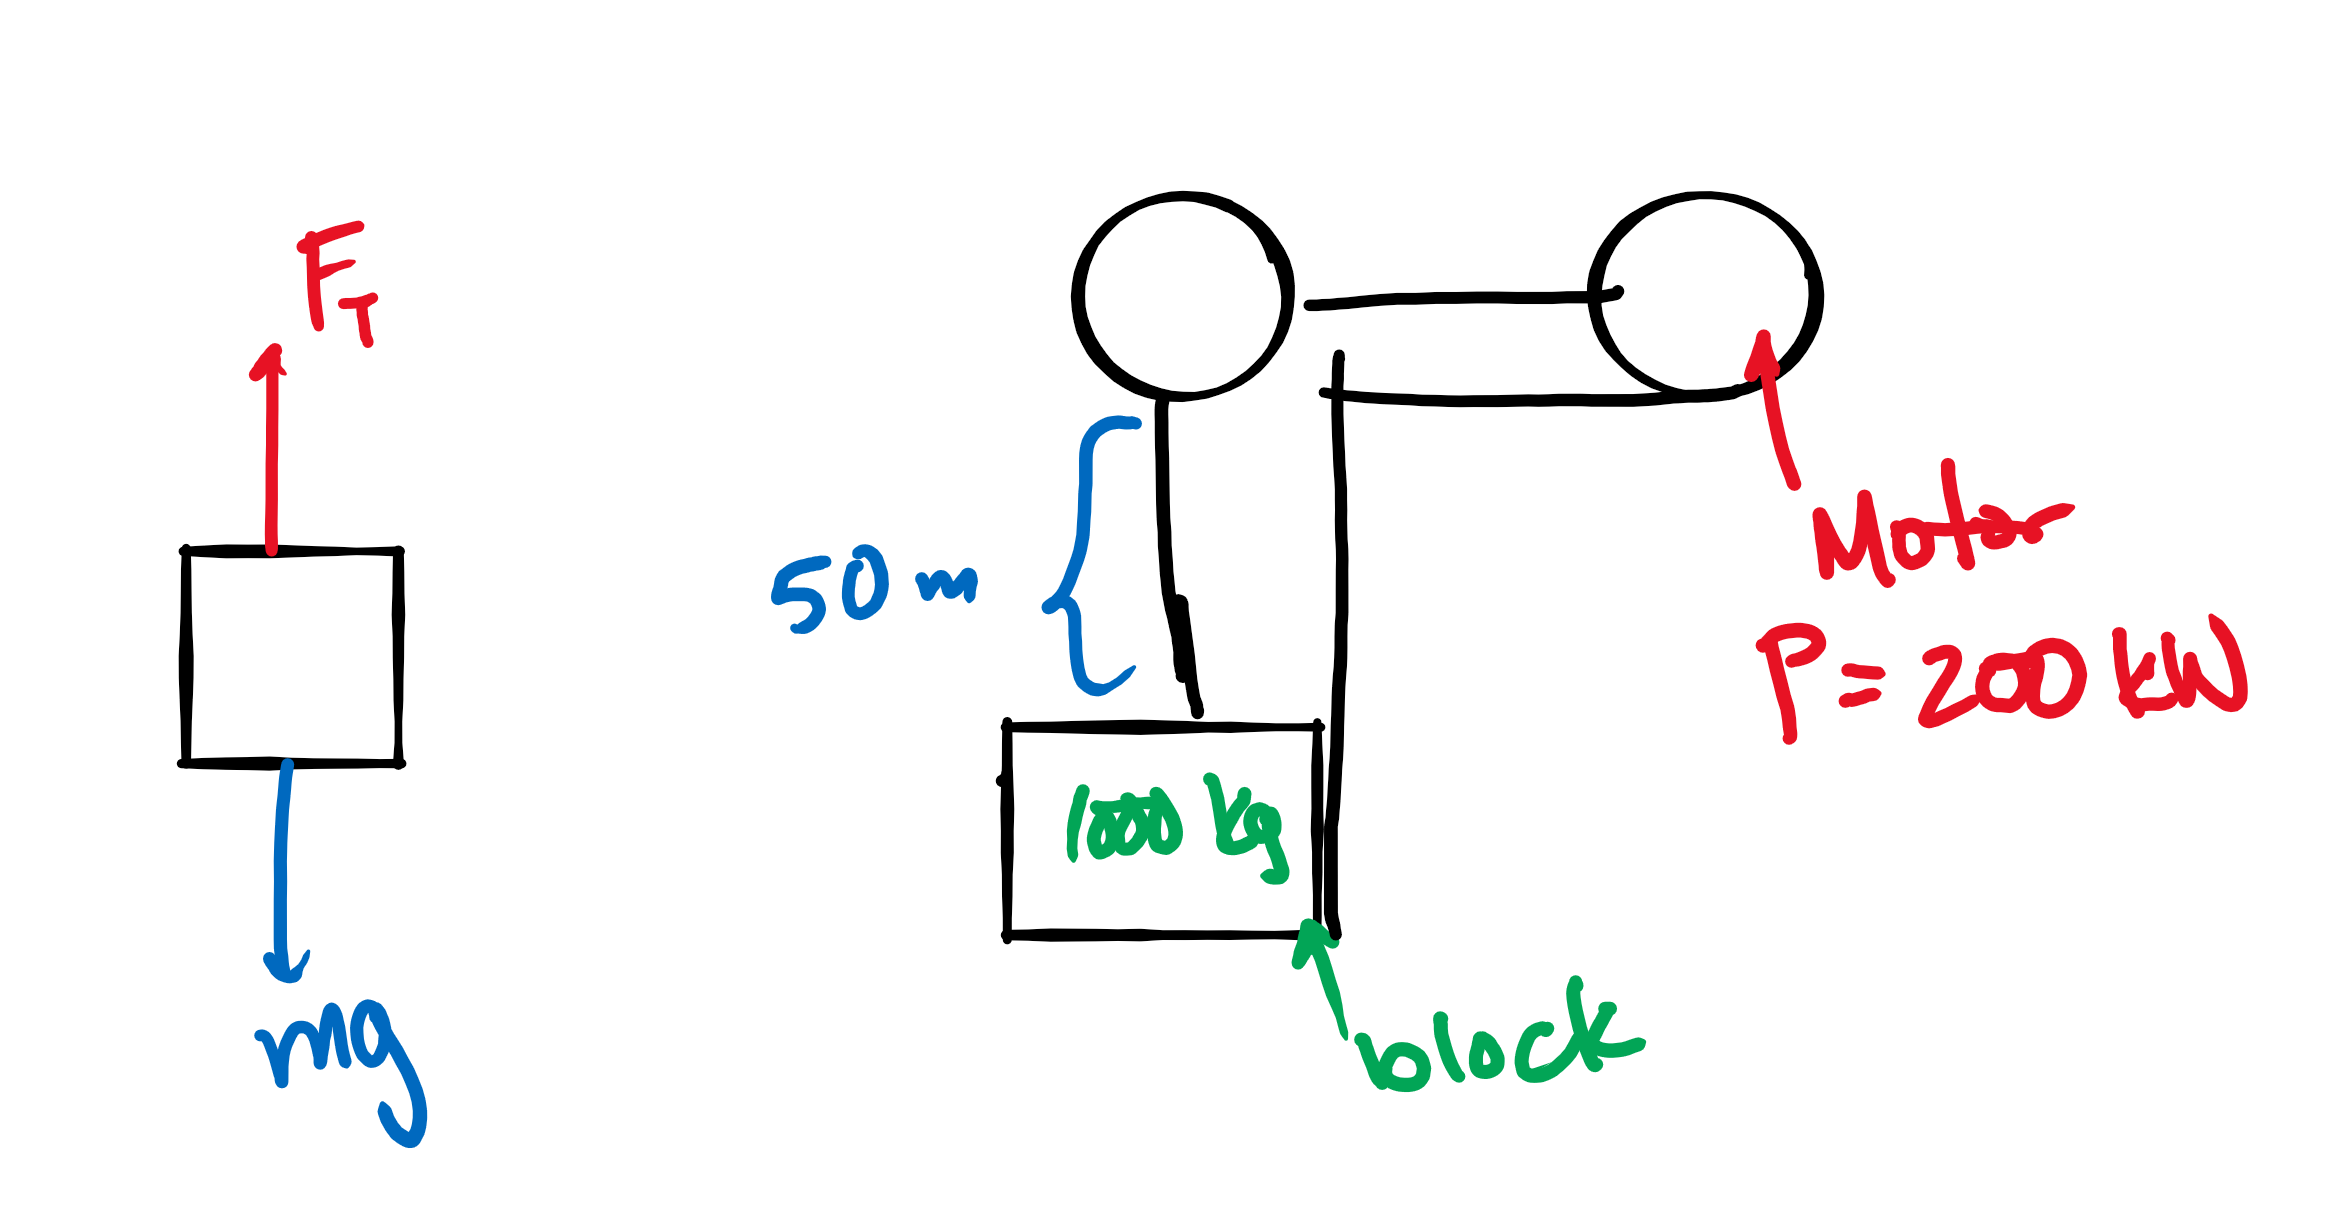
\includegraphics[width=0.5\textwidth]{chapters/ch4/images/fig4_8}
    \end{center}

    $$
    \begin{aligned}
        P &= \frac{\Delta E}{\Delta t}\\
        P &= \frac{\Delta KE + \Delta PE}{\Delta t}\\
        P &= \frac{\frac{1}{2}mv^2+mgh}{\Delta t}\\
        v_f &= \sqrt{\frac{2(-mgh+\Delta T P)}{m}}
    \end{aligned}
    $$
\end{problem}


\begin{problem}
    A truck drives up a ramp with an angle of inclination of $15^\circ$. If the truck drives 200 meters in 20 seconds, what is the power of the truck (in kW) after the truck has moved 200 meters? Assume that 10\% of the total energy is lost to the environment.

    $$
    \begin{aligned}
        P &= \frac{\Delta E}{t}\\
        P &= \frac{\Delta KE + \Delta PE}{t}+ 10\%\text{ energy}\\
        P &= \frac{\frac{1}{2}mv^2 + mgh}{t} + 10\%\text{ energy}\\
        P &= \left[\frac{\frac{1}{2}m\left(\frac{\Delta x}{t}\right)^2 + mgL\sin\theta}{t}\right]\frac{1}{0.9}\\
        P &= 98.3 \text{ kW}
    \end{aligned}
    $$
\end{problem}


\begin{problem}
    A person with mass 80 kg is on a scooter on top of a hill that is 30 m tall. The person is pushed off by a spring with a spring coefficient of 1500 N/m. The spring is compressed 2.5 m. The person will then go down a hill and launch into the air, then land in a pit of tar with a coefficient of kinetic friction of 0.8. \\

    a) Find the velocity of the person right after the spring pushes him off.\\

    b) Find the distance the person will travel after he lands in the tar. 

    \begin{center}
        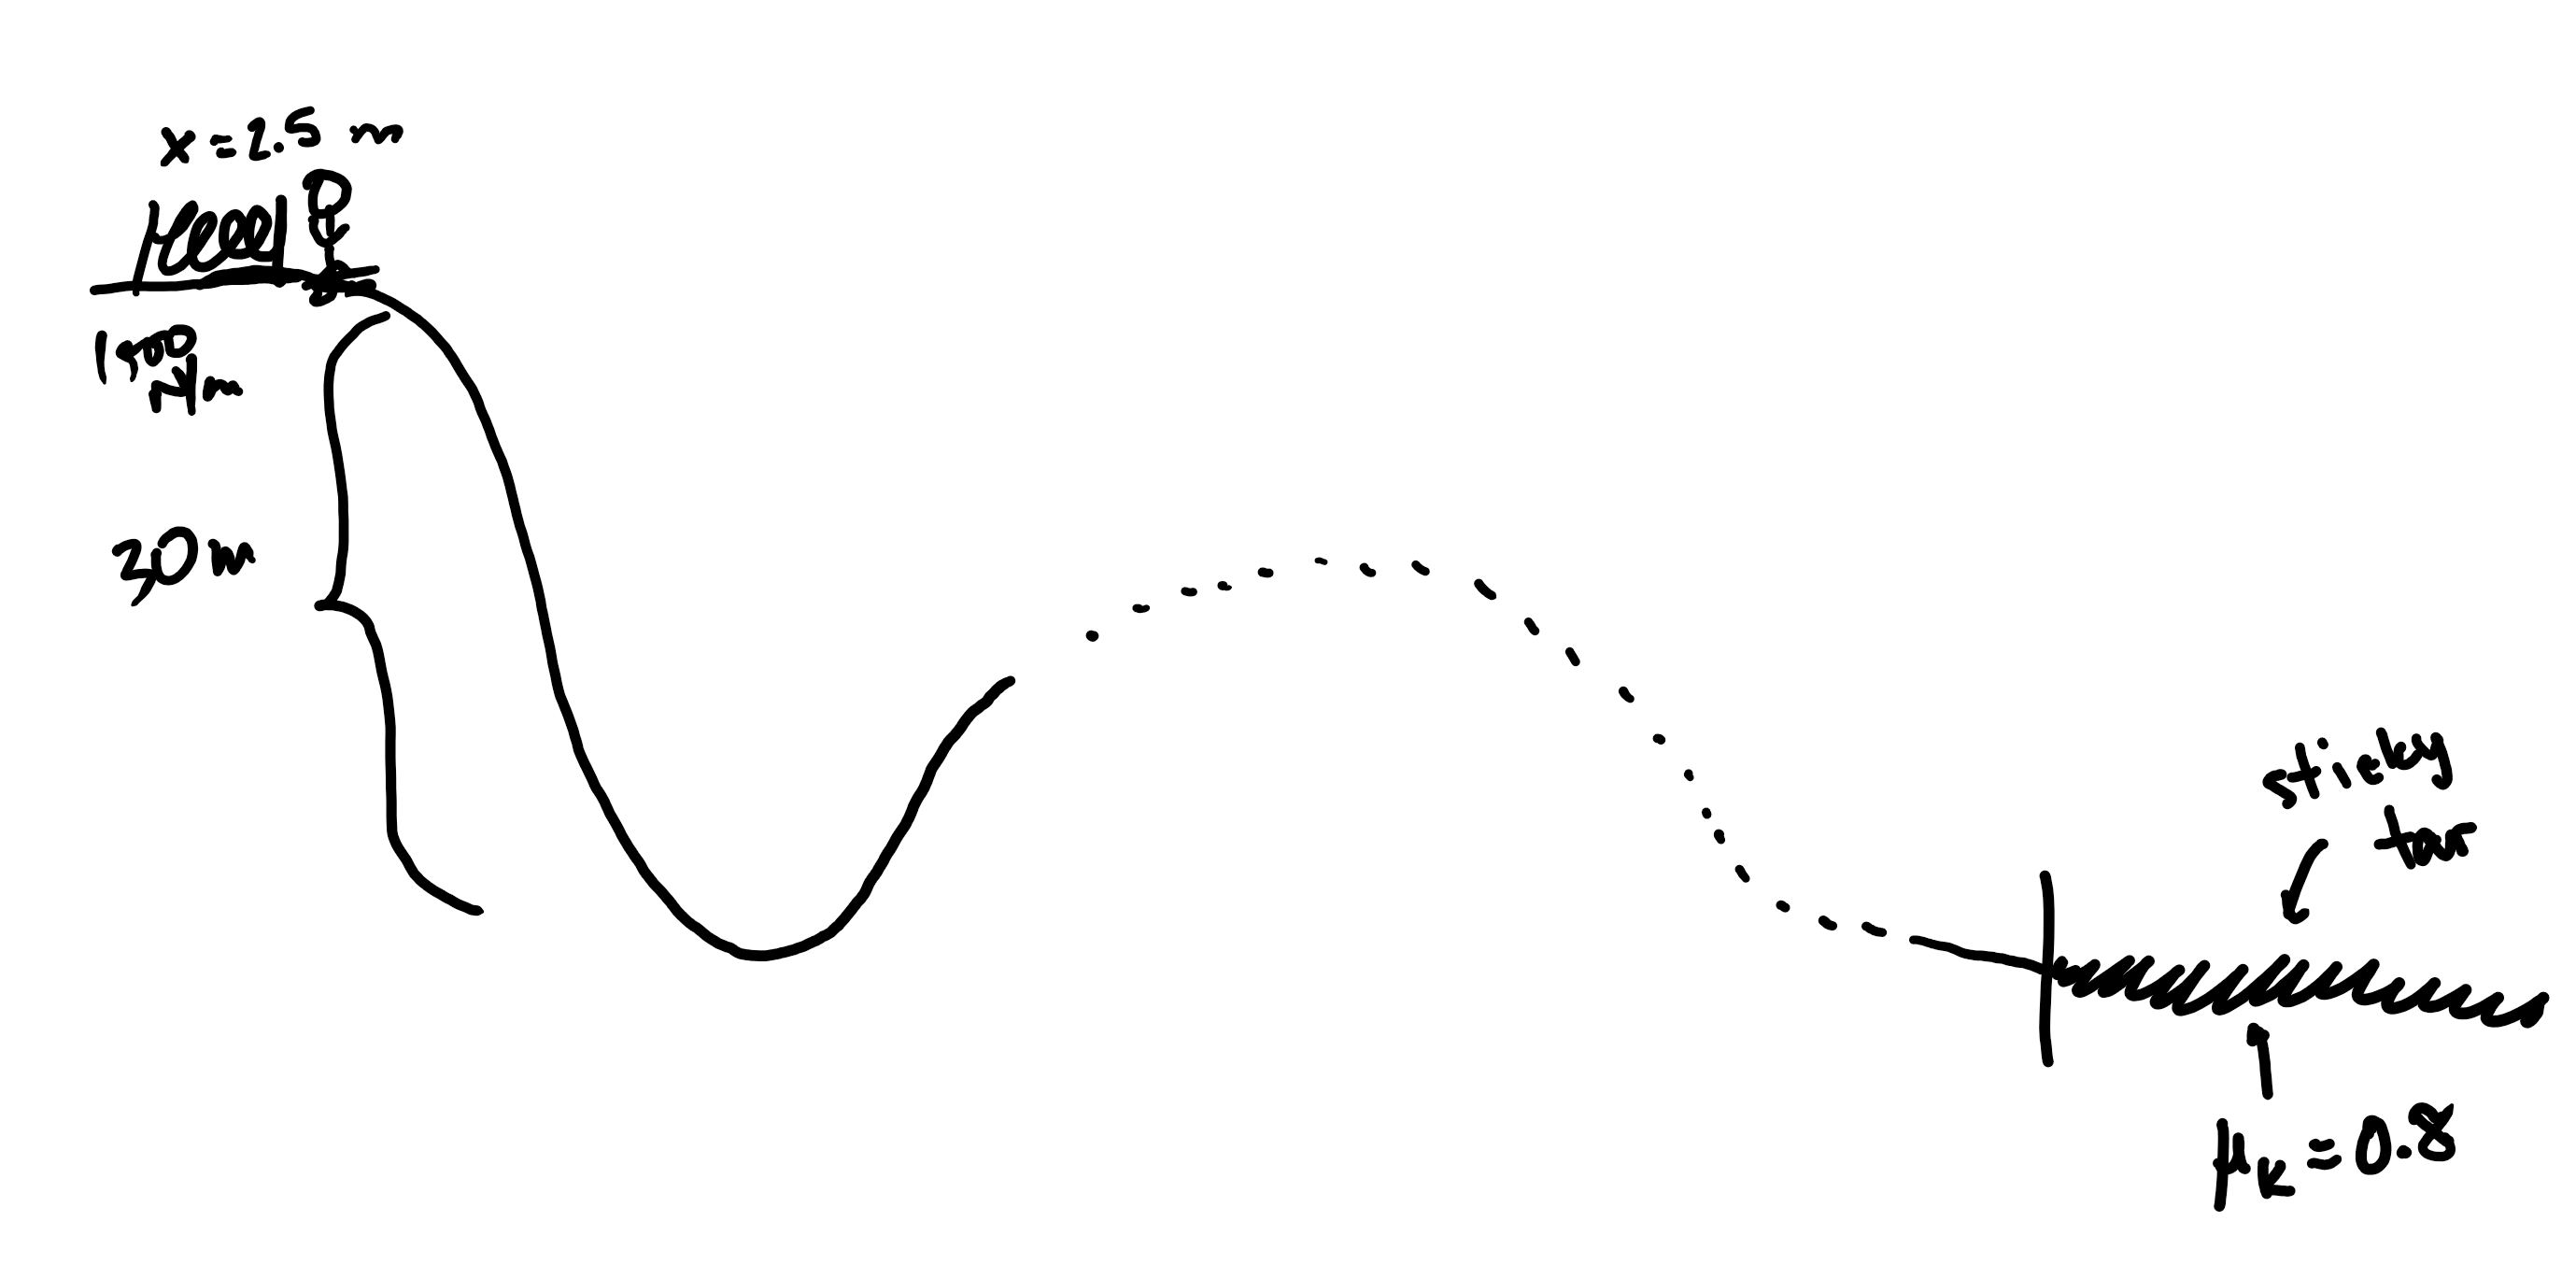
\includegraphics[width=0.75\textwidth]{chapters/ch4/images/fig4_10.PNG}
    \end{center}

    a)

    $$
    \begin{aligned}
        W &= \Delta KE + \Delta E_s\\
        0 &= \frac{1}{2}mv_i^2+\frac{1}{2}k(-x_i)^2\\
        v_i = \sqrt{\frac{kx_i^2}{m}}\\
        v_i = 10.8 \frac{\m}{\s}
    \end{aligned}
    $$

    b)
    $$
    \begin{aligned}
        W &= -\frac{1}{2}m(v_i)^2 + mg(-h_i) + F_fd\\
        0 &= -\frac{1}{2}mv_i^2 + - mgh_i + \mu_kF_Nd\\
        d &= \frac{mgh_i + \frac{1}{2}mv_i^2}{\mu_kmg}\\
        d &= 44.9 \m
    \end{aligned}
    $$
\end{problem}


\begin{problem}
    A ball with mass 2 kg is placed inside a cannon that is launched using a spring with spring constant 200 N/m. The spring is compressed 2 m and is compressed all the way to the ground (so that $PE_i = 0$). The cannon is at an angle of $20^\circ$. What is the maximum height that the ball is launched?

    \begin{center}
        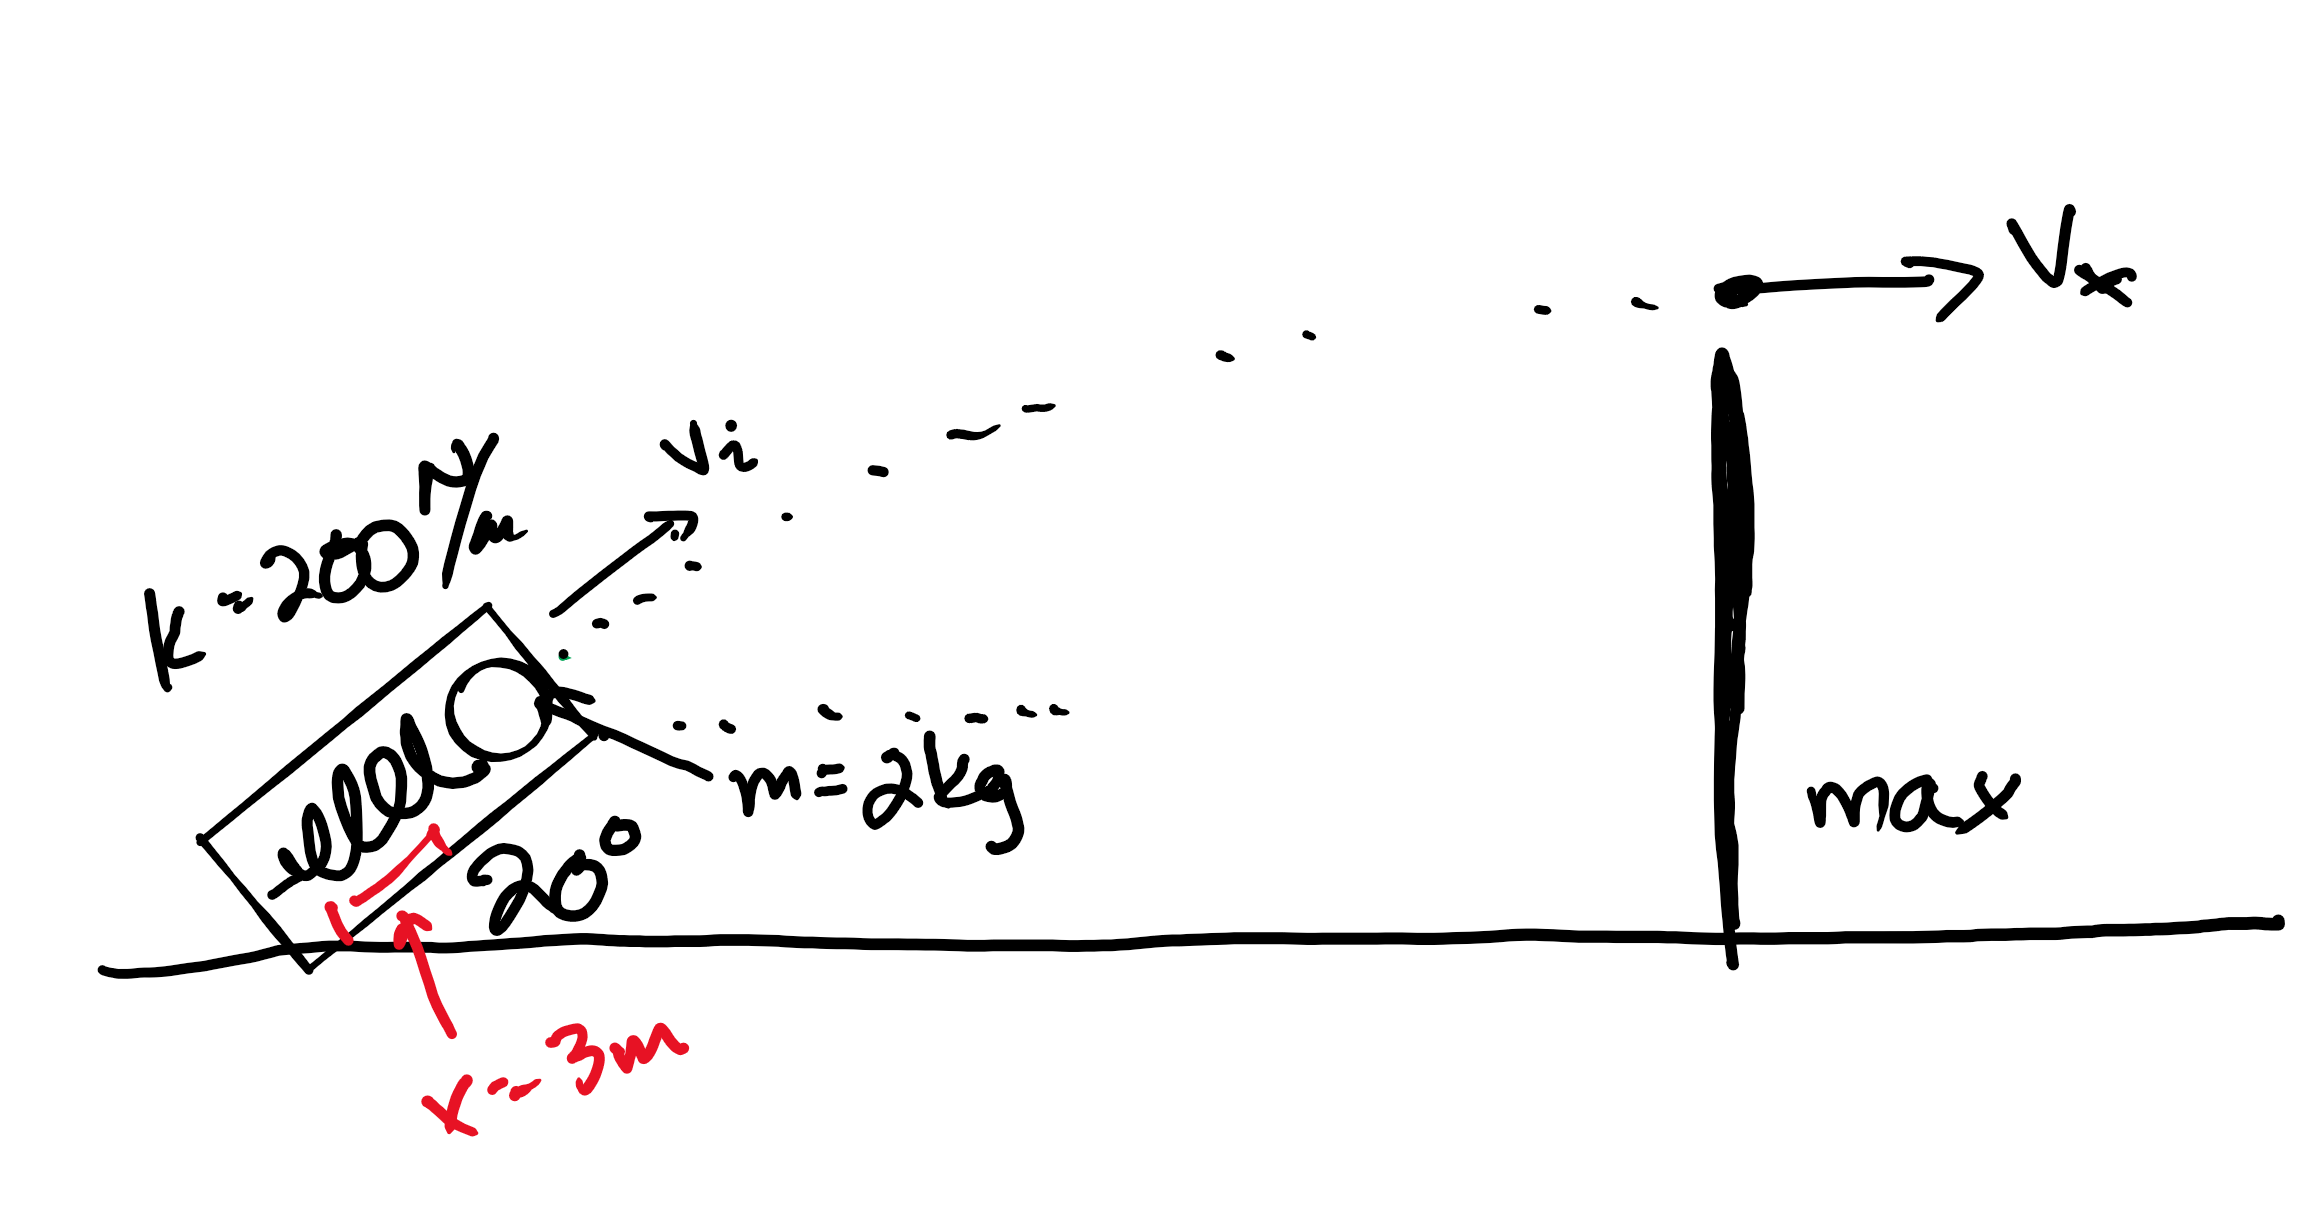
\includegraphics[width=0.75\textwidth]{chapters/ch4/images/fig4_11.PNG}
    \end{center}

    We first need the velocity right when the ball leaves the spring. We can set up a mini Work-Energy problem:
    $$
    \begin{aligned}
        W &= \Delta KE + \Delta PE + \Delta E_s\\
        0 &= \frac{1}{2}mv_i^2 + mgL\sin\theta + \frac{1}{2}k(-(L^2))\\
        \frac{1}{2}mv_i^2 &= \frac{1}{2}kL^2 - mgl\sin\theta\\
        v_i &= \sqrt{\frac{2\left(\frac{1}{2}kL^2 - mgl\sin\theta\right)}{m}}
    \end{aligned}
    $$


    Now we can use the x-component of that velocity to get the final velocity in the overall Work-Energy problem.
    $$
    \begin{aligned}
        W &= \Delta KE + \Delta PE + \Delta E_s\\
        0 &= \frac{1}{2}mv_x^2 + mgh_f + \frac{1}{2}k(-(x^2))\\
        mgh_f &= \frac{1}{2}mv_x^2 -\frac{1}{2}kx^2\\
        h_f &= \frac{\frac{1}{2}mv_x^2 -\frac{1}{2}kx^2}{mg}
    \end{aligned}
    $$
\end{problem}


\section{Non-Conservative Energy}

Not all energy is conserved and remained in the system - sometimes the energy is lost to the environment as thermal energy and sound energy


\begin{problem}
    A skiier skiis down a ramp in two parts. On the first part, the angle of elevation is $30^\circ$ and the kinetic coefficient of friction is 0.2. Once the skiier reaches the bottom of the slope, the new coefficient of kinetic friction is 0.3. The slope is 70m tall.\\

    a) What is the velocity of the skiier at the bottom of the slope?\\

    b) What is the acceleration of the skiier while he is on the slope?\\

    c) What is the distance the skiier will slide once he hits the bottom of the slope?\\

    To solve part a):
    $$
    \begin{aligned}
        W &= \Delta KE + \Delta PE + \Delta E_s + E_{TH}\\
        0 &= \frac{1}{2}m(v_f^2-0) + mg(0-h_i) + F_f\cdot\frac{h_i}{\sin\theta}\\
        v_f^2 &= 2\left(gh_i - g\cos\theta\mu_k\frac{h_i}{\sin\theta}\right)\\
        v_f &= \sqrt{2\left(gh_i - g\cos\theta\mu_k\frac{h_i}{\sin\theta}\right)}\\
        v_f &= \sqrt{2gh_i\left(1 - \frac{\mu_k}{\tan\theta}\right)}\\
        v_f &= 36.374 \frac{\m}{\s}
    \end{aligned}
    $$

    To solve part b):
    $$
    \begin{aligned}
        v_f^2 = v_i^2 + 2aL\\
        a = \frac{v_f^2}{2L}\\
        a = \frac{\m}{\s^2}
    \end{aligned}
    $$

    To solve part c):
    $$
    \begin{aligned}
        W &= \Delta KE + \Delta PE + \Delta E_s + E_{TH}\\
        0 &= \frac{1}{2}m(-v_i^2)+F_fD\\
        D &= \frac{v_i^2}{2\mu_kg}\\
        D &= 240.619\m
    \end{aligned}
    $$
\end{problem}


\begin{problem}
    A rock with mass 10kg falls 5m onto a spring with spring constant 100 N/m. What is the the distance that the spring compresses due to the rock falling onto the spring?\\
    
    INCLUDE FIGURE HERE\\

    $$
    \begin{aligned}
        W &= \Delta KE + \Delta PE + \Delta E_s + E_{TH}\\
        0 &= \Delta PE + \Delta E_s\\
        0 &= mg(0-(h+y))+\frac{1}{2}k(y^2-0)\\
        \text{FINISH THIS PROBLEM LATER}
    \end{aligned}
    $$
\end{problem}


\begin{problem}
    INSERT TEXT ABOUT THE PROBLEM HERE

    \begin{center}
        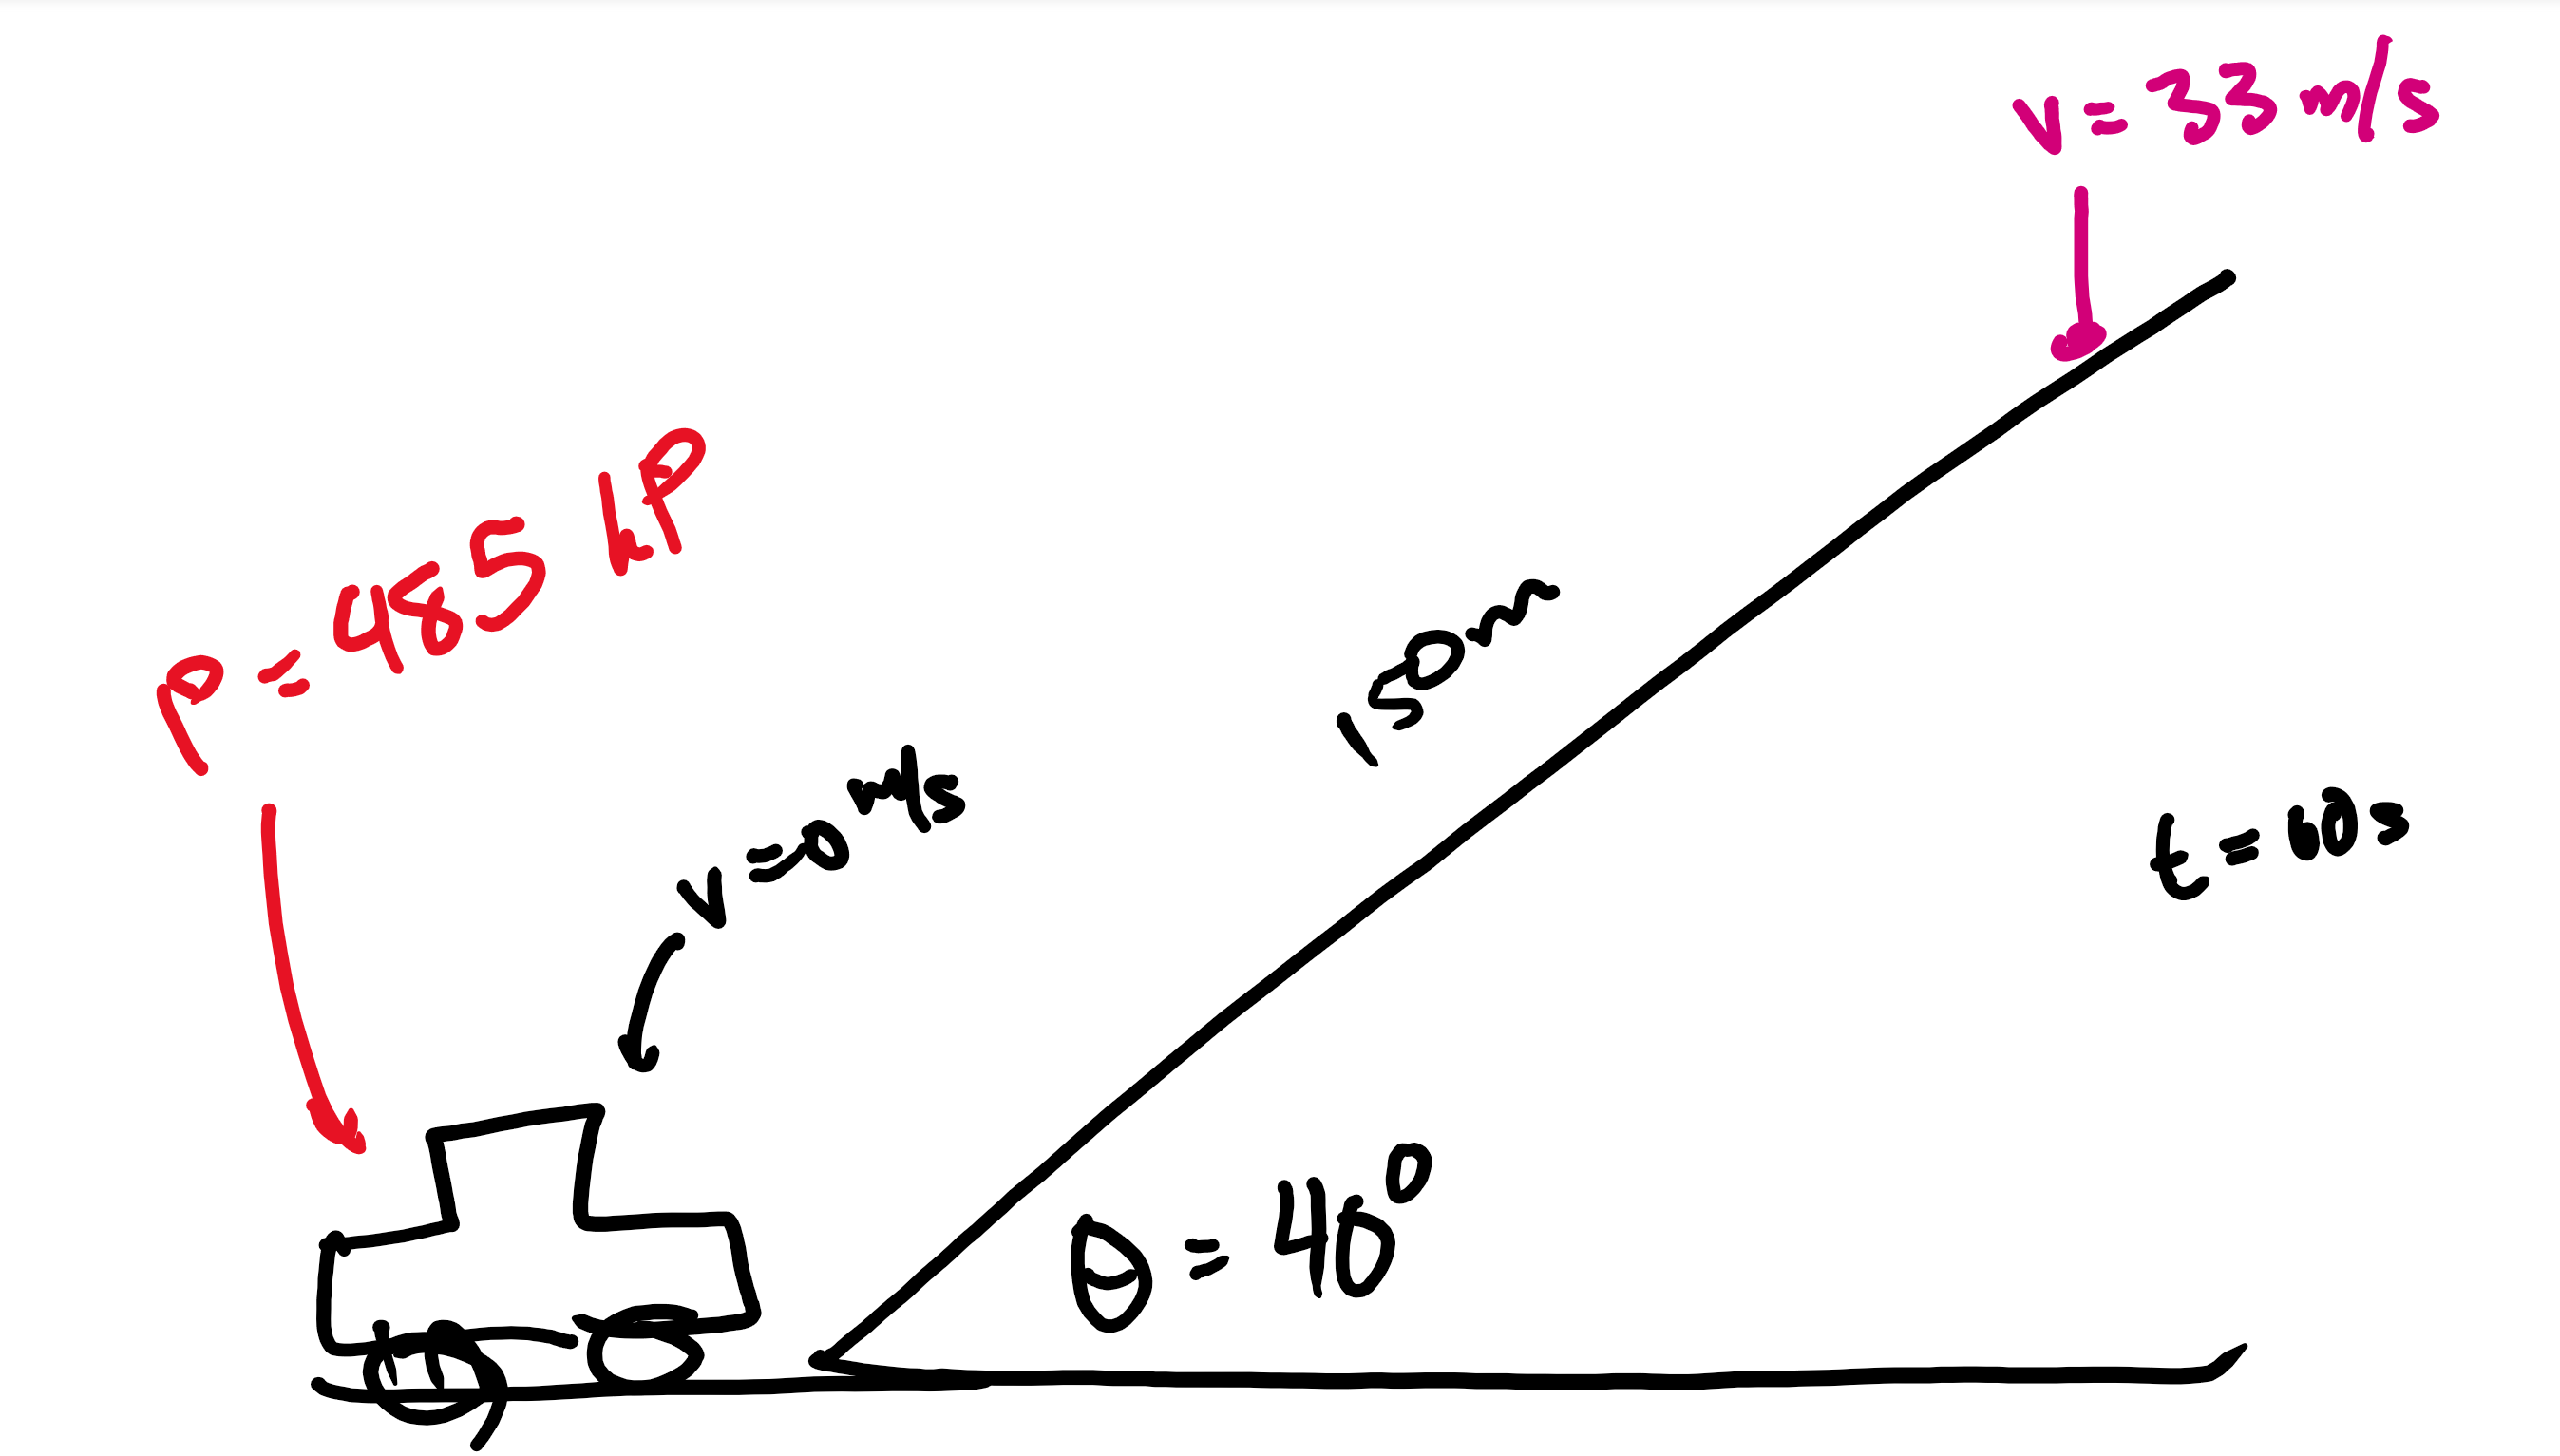
\includegraphics[width=0.75\textwidth]{chapters/ch4/images/fig4_13.PNG}
    \end{center}

    $$
    \begin{aligned}
        W &= \Delta KE + \Delta PE +\Delta E_s + E_{TH}\\
        E_{TH} &= W - \Delta KE - \Delta PE\\
        E_{TH} &= Pt - \Delta KE - \Delta PE\\
        E_{TH} &= Pt - \frac{1}{2}mv_f^2 - mgd\sin\theta
    \end{aligned}
    $$
\end{problem}



\section{Center of Mass}

\begin{itemize}
    \item A lot of times we are looking at an entire system with a bunch of different objects spread throughout
    \item If this is the case, we want to know where all of the mass for every single object (on average) is concentrated
    \item Finding the point where most of the mass is cnocentrated is called the \textbf{center of mass}
\end{itemize}

\begin{definition}[Center of Mass (1D)]{def4.6.1:label}
    If there are multiple masses $m_1,m_2\dots,m_n$ that are all in 1D space, then the center of mass can be determined using the following equation:

    \[
        m_{c} = \frac{\sum_{i=0}^n m_ix_i}{\sum_{i=0}^n m_i}    
    \]

    Where $x_i$ is the position value for the indicated mass.
\end{definition}


\newpage
\begin{definition}[Center of Mass (2D)]{def4.6.2:label}
    If there are multiple masses $m_1,m_2\dots,m_n$ that are all in 2D space, then the center of mass can be determined using the following equations:

    \[
        \begin{aligned}
            m_{xc} &= \frac{\sum_{i=0}^n m_ix_i}{\sum_{i=0}^n m_i}\\
            m_{yc} &= \frac{\sum_{i=0}^n m_iy_i}{\sum_{i=0}^n m_i} 
        \end{aligned}   
    \]

    Where $x_i$ is the x-position of the indicated mass and $y_i$ is the y-position of the indicated mass.
\end{definition}


\section{Introduction to Momentum}

\begin{definition}[Momentum]{def4.7.1:label}
    \[
    \vec p = m \vec v  
    \]

    \textbf{momentum} is a vector (it's simply a scaled version of velocity) and the SI units are $\kg \frac{\m}{\s}$.
\end{definition}

\begin{itemize}
    \item linear momentum is \textbf{always conserved}
    \item kinetic energy is only conserved in an \textbf{elastic collision}
    \begin{itemize}
        \item \textit{ELASTIC COLLISION}: Where two bodies bounce off of each other
        \item \textit{INELASTIC COLLISION:} When two bodies stick together after the collision
    \end{itemize}
    \item FUN FACT: We can get Newton's second law through differentiating the definition of momentum because $\frac{d}{dt}p = \frac{d}{dt}(mv) \implies F_{net} = ma$
\end{itemize}

\begin{definition}[Impulse]{def4.7.2:label}
    \[
    \vec J = \vec Ft = \Delta \vec p = m(\vec v_f - \vec v_i)
    \]

    \textbf{impulse} is how much is applied to an object over a given period of time
\end{definition}

\begin{itemize}
    \item NOTE: Impulse is the \textbf{area under a Force vs time graph}
\end{itemize}


\begin{problem}
    If a baseball comes in to the left at $50 \frac{\m}{\s}$ and gets hit back to the right with a velocity of $80 \frac{\m}{\s}$ at an angle of $30^\circ$. If the right direction is positive, what is the time interval during which the collision of the ball occurred?

    \[
    \begin{aligned}
        F_{avg}t &= m(v_f-v_i)\\
        F_{avg} &= \frac{m(v_f-v_i)}{t}\\
        F_{avg} &= \frac{m<v_{fx} - v_{ix}, v_{fy}-v_{iy}>}{t}\\
        F_{avg} &= 328.6 \vec i + 80 \vec j = 251.6 \angle 18.5^\circ
    \end{aligned}    
    \]
\end{problem}


\begin{problem}
    A cue ball comes and towards the 6-ball with a speed of $2 \frac{\m}{\s}$. The 6-ball goes down at an angle of $30^\circ$ with a velocity magnitude of $3 \frac{\m}{\s}$. What is the final velocity of the cue ball after the collision?
    
    \[
    \begin{aligned}
        \vec p_i &= \vec p_f\\
        m\vec v_{ci} &= m\vec v_{cf} + m\vec v_6\\
        v_{cf} &= v_{ci}-v_6\\
        v_{cf} &= 2\vec i - (2.6 \vec i - 1.5 \vec j)\\
        v_{cf} &= -0.6\vec i + 1.5 \vec j\\
        v_{Cf} &= 1.62 \angle 62.5^\circ \frac{\m}{\s}
    \end{aligned}  
    \]

    NOTE: You can also choose to solve for the momentums in each direction independently (so say that $p_{xi} = p_{xf}$ and then also $p_{yi} = p_{yf}$ and then solve both individually).
\end{problem}